\documentclass[10pt, ucs, notheorems, handout]{beamer}

\usetheme[numbers,totalnumbers,minimal,nologo]{Statmod}
\usefonttheme[onlymath]{serif}
\setbeamertemplate{navigation symbols}{}
\setbeamercolor{alerted text}{fg=blue}
\usepackage{physics}

\mode<handout> {
    \usepackage{pgfpages}
    %\setbeameroption{show notes}
    %\pgfpagesuselayout{2 on 1}[a4paper, border shrink=5mm]
    \setbeamercolor{note page}{bg=white}
    \setbeamercolor{note title}{bg=gray!10}
    \setbeamercolor{note date}{fg=gray!10}
}

\usepackage[utf8x]{inputenc}
\usepackage[T2A]{fontenc}
\usepackage[english, russian]{babel}
\usepackage{tikz}
\usepackage{ragged2e}
\usepackage{graphicx}
\usepackage{subfigure}


\usepackage{latexsym,amssymb}
\usepackage{amsmath}
\usepackage{amsfonts}
\usepackage{amsthm}

\DeclareMathOperator{\rk}{rk}
\DeclareMathOperator{\med}{med}
\DeclareMathOperator{\diag}{diag}
\DeclareMathOperator*{\argmin}{argmin}
\newcommand{\tX}[1]{\mathsf{#1}}
\newcommand{\iu}{\mathrm{i}\mkern1mu}
\newcommand{\RomanNumeralCaps}[1]
{\MakeUppercase{\romannumeral #1}}

\title[Робастные варианты метода SSA]{%
	Робастные варианты метода SSA}

\author{Сенов Михаил Андреевич}

\institute[СПбГУ]{Санкт-Петербургский государственный университет \\
	%Математико-механический факультет \\
	%Кафедра статистического моделирования \\
	Уровень образования: бакалавриат\\
	Направление 01.03.02 <<Прикладная математика и информатика>>\\
	Основная образовательная программа СВ.5004.2018 <<Прикладная математика и информатика>> \\
	Профессиональная траектория <<Вычислительная стохастика и статистические модели>>\\
	\vspace{0.4cm}
	Научный руководитель: к.ф.-м.н., доц. Голяндина Н.Э. \\
	Рецензент: к.ф.-м.н. Пепелышев А.Н.
	\vspace{0.3cm}
}

\date[Защита]{Санкт-Петербург, 2022}

\begin{document}

\begin{frame}
  \titlepage
  \note{}
\end{frame}

\begin{frame}{Введение}

$\tX{X} = (x_1, \ldots, x_{N})$ временной ряд длины $N$.\\
\vspace{1em}
\alert{Модель:} $\tX{X} = \tX{S} + \tX{R}$, $\tX{S}$ сигнал, $\tX{R}$ возмущение (шум или выброс).\\
\vspace{1em}
\alert{Задача:} Оценить сигнал $\tilde{\tX{S}} = F(\tX{X})$, $F$ --- используемый метод.\\
\vspace{1em}
\alert{Метод:} SSA (Singular Spectrum Analysis) [Golyandina et al., 2001] для вещественных рядов, CSSA (Complex Singular Spectrum Analysis) --- обобщение для комплексных рядов.\\
\vspace{1em}
\alert{Проблемы:}
\begin{enumerate}
	\item Разработаны робастные модификации SSA (Третьякова, 2020). Робастные модификации CSSA? 
	\item Что лучше, с точки зрения величины ошибки $\tilde{\tX{S}} - \tX{S}$,\\
	SSA$(\tX{X}_{\Re}) + \iu \text{SSA}(\tX{X}_{\Im})$ или CSSA$(\tX{X}_{\Re} + \iu \tX{X}_{\Im})$?
\end{enumerate} 

\end{frame}

\begin{frame}{Часть \RomanNumeralCaps{1}: Введение}
	Базовый SSA: реагирует на выбросы.
	\begin{center}
		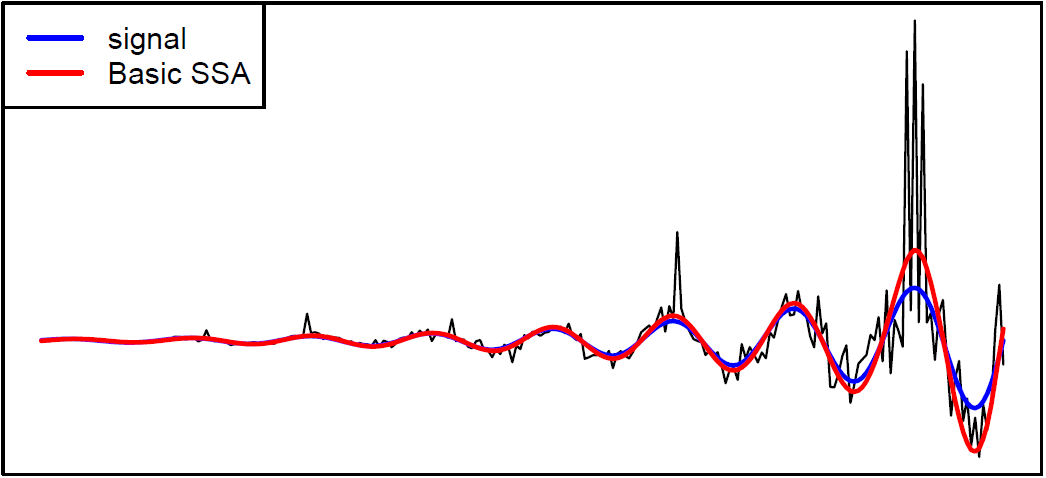
\includegraphics[, height = 3cm]{img/otliers_ssa.PNG}
	\end{center}
	
	Робастный SSA: не реагирует на выбросы.
	\begin{center}
		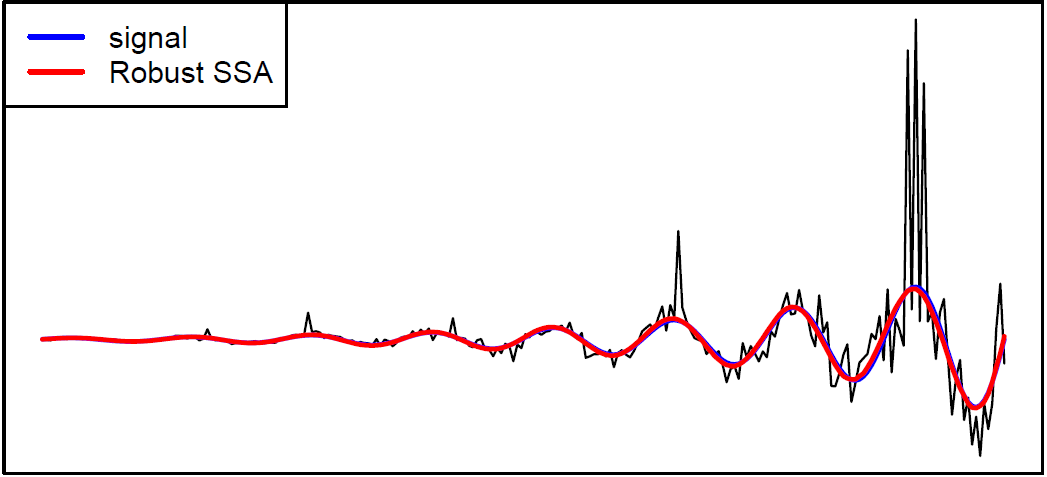
\includegraphics[, height = 3cm]{img/outliers_l1.PNG}
	\end{center}
	
	\note{}
\end{frame}

%\begin{frame}{Введение: Цель работы}
%	Робастный SSA разработан для вещественных временных рядов.\\
%	\vspace{1em}
%	\alert{Цель:} Обобщить временной ряд на комплексный случай.\\
%	\vspace{1em}
%	Распространённый пример комплексного временного ряда~--- это инженерные задачи, где данные получаются путём преобразования Фурье.
%	$$\tX{X}_N^{(t)} = (x_1^{(t)}, \ldots, x_N^{(t)}), \, t = 1 \ldots M,$$
%	$$\tX{DFT}(\tX{X}_N^{(t)}) = f^{(t)}_k = \sum_{n=1}^{N}x^{(t)}_n e^{-2 \pi i k  n / N}, \, k = 1 \ldots N,$$
%	$$\tX{F}^{(M)}_{k} = (f^{(1)}_k, \ldots, f^{(M)}_k).$$
%\end{frame}


\begin{frame}{Часть \RomanNumeralCaps{1}: Обозначения}
	Рассмотрим временной ряд $\tX{X}=(x_1, \ldots, x_{N})$, $L$ длина окна, $K=N-L+1$.\\
	\vspace{1em}
	$\mathcal{M}_{r}$ --- пространство матриц размера $L \times K$ ранга не больше $r$.
	
	$\mathcal{M}_{\mathcal{H}}$~--- пространство ганкелевых матриц $L\times K$.\\
	\vspace{1em}
	Оператор вложения $\mathcal{T}_L:\mathbb{R}^N \rightarrow \mathcal{M}_{\mathcal{H}}: \mathcal{T}_L (\tX{X}) = \mathbf{X} $,\\
	$$\mathbf{X} = \begin{pmatrix}
		x_1 & x_2 & \ldots & x_{K}\\
		x_2 & x_3 & \ldots & x_{K+1}\\
		\vdots & \vdots & & \vdots\\
		x_{L} & x_{L+1} & \ldots & x_{N}
	\end{pmatrix}, K = N - L + 1,$$
	$\mathbf{X}$~--- $L$-траекторная матрица $\tX{X}$.\\
	\vspace{1em}
	$\Pi_{r}:\mathcal{M}\rightarrow \mathcal{M}_r$,
	$\Pi_{\mathcal{H}}:\mathcal{M} \rightarrow \mathcal{M}_{\mathcal{H}}$~--- проекторы на $\mathcal{M}_{r}$ и $\mathcal{M}_{\mathcal{H}}$ по норме Форбениуса.
	
	\note{}
	
\end{frame}

\begin{frame}{Часть \RomanNumeralCaps{1}: Выделение сигнала}
	
	Временной ряд $\tX{X}_N=(x_1, \ldots, x_{N})$.
	\begin{block}{Алгоритм для выделения сигнала}
		\begin{equation*}
			\tilde{\tX{S}} = \mathcal{T}_L^{-1} \Pi_{\mathcal{H}} \Pi_{r} \mathcal{T}_L (\tX{X_N}).
		\end{equation*}
	\end{block}
	
	
	Нормы для $\Pi_r$ и $\Pi_{\mathcal{H}}$:
	\begin{itemize}
		\item $\mathbb{L}_2$(Фробениус): выделение сигнала базовым SSA
		$$\|\mathbf{X}\|_\mathrm{F} = \sqrt{\sum_{i = 1}\sum_{j = 1}|x_{ij}|^2}.$$
		\item $\mathbb{L}_1$: робастная версия SSA
		$$\|\mathbf{X}\|_1 = \sum_{i = 1}\sum_{j = 1}|x_{ij}|.$$
		\item weighted $\mathbb{L}_2$ : робастная версия SSA
		$$\|\mathbf{W}^{1/2}\odot\mathbf{X}\|_\mathrm{F} = \sqrt{\sum_{i = 1}\sum_{j = 1}w_{ij}|x_{ij}|^2}.$$
	\end{itemize}
	\note{}
\end{frame}

%\begin{frame}{Методы: Иллюстрирующий пример}
%	\begin{block}{Пример}
%		$(x_1, \ldots, x_N)$, норма $p(x)$, $\argmin\limits_{c}p((x_1 - c, \ldots, x_N - c)) =\, ?$
%	\end{block}
%	Нормы:
%	\begin{itemize}
%		\item $\mathbb{L}_2$. $\overline{x} = \argmin\limits_{c} \sqrt{\sum_{i = 1}^{N} |x_i - c|^2}$. \\
%		Если $x_j \to \infty$, тогда $\overline{x} \to \infty$. Не робастный.
%		\item $\mathbb{L}_1$. $\med = \argmin\limits_{c} \sum_{i = 1}^{N} |x_i - c|$. \\
%		Если $x_j \to \infty$, тогда $\med \not\to \infty$. Робастный.
%		\item weighted $\mathbb{L}_2$. $\overline{x}_w = \argmin\limits_{c} \sqrt{\sum_{i = 1}^{N} w_i|x_i - c|^2}$.\\
%		Если $x_j \rightarrow \infty$, тогда возьмём $w_i = 0$ и $\overline{x}_w \not\to \infty$. Робастный.
%	\end{itemize}
%\end{frame}

\begin{frame}{Часть \RomanNumeralCaps{1}: Результаты}
	Траекторная матрица $\mathbf{Y} \in \mathbb{C}^{L\times K}$ на вход.\\ 
	Обозначим $\mathbf{M} \in \mathbb{C}^{L\times r}, \mathbf{V} \in \mathbb{C}^{K\times r}, \mathbf{W} \in \mathbb{R}^{L\times K}$.\\
	\vspace{1em}
	Алгоритмы, решающие следующие задачи, были реализованы на языке R:
	\begin{itemize}
		\item $\mathbb{L}_2$ CSSA: 
		$$ \|\mathbf{Y}-\mathbf{M}\mathbf{V}^{\mathrm{H}}\|_\mathrm{F} \longrightarrow \min_{\mathbf{M},\mathbf{V}},$$
		имеет точное решение.
		\item $\mathbb{L}_1$ CSSA:
		$$\|\mathbf{Y}-\mathbf{M}\mathbf{V}^{\mathrm{H}}\|_1 \longrightarrow \min_{\mathbf{M},\mathbf{V}}.$$
		решение вычисляется итеративно.
		\item weighted $\mathbb{L}_2$ CSSA:
		$$\|\mathbf{W}^{1/2}\odot(\mathbf{Y}-\mathbf{M}\mathbf{V}^{\mathrm{H}})\|_\mathrm{F} \longrightarrow \min_{\mathbf{M},\mathbf{V}},$$
		решение вычисляется итеративно, $\mathbf{W}$ обновляется на каждой итерации. 
	\end{itemize}

\end{frame}

\begin{frame}{Часть \RomanNumeralCaps{2}: Введение}
	
	$\tX{X} = (x_1, \ldots, x_{N})$ временной ряд длины $N$.\\
	\vspace{1em}
	\alert{Модель:} $\tX{X} = \tX{S} + \tX{R}$, $\tX{S}$ сигнал, $\tX{R}$ возмущение (шум или выброс).\\
	\vspace{1em}
	\alert{Задача:} Оценить сигнал $\tilde{\tX{S}} = F(\tX{X})$, $F$ --- используемый метод.\\
	\vspace{1em}
	\alert{Метод:} SSA (Singular Spectrum Analysis) [Golyandina et al., 2001] для вещественных рядов, CSSA (Complex Singular Spectrum Analysis) --- обобщение для комплексных рядов.\\
	\vspace{1em}
	\alert{Проблема:} Что лучше, с точки зрения величины ошибки $\tilde{\tX{S}} - \tX{S}$,\\
	SSA$(\tX{X}_{\Re}) + \iu \text{SSA}(\tX{X}_{\Im})$ или CSSA$(\tX{X}_{\Re} + \iu \tX{X}_{\Im})$?\\
	\vspace{1em}
	Рассматриваем теорию возмущений (Kato, 1966). Будем вычислять первый порядок ошибки (Nekrutkin, 2008), в предположении, что он достаточно точно описывает полную ошибку.
\end{frame}


\begin{frame}{Часть \RomanNumeralCaps{2}: Обозначения}
Временной ряд $\tX{X}=(x_1, \ldots, x_{N})$, $L$ --- длина окна, $r$ --- ранг оцениваемого сигнала (ранга траекторной матрицы сигнала).
    \begin{block}{Алгоритм SSA (CSSA) выделения сигнала}
\begin{equation*}
	\tilde{\tX{S}} = \mathcal{T}^{-1}_{L} \Pi_{\mathcal{H}} \Pi_{r} \mathcal{T}_L (\tX{X}).
\end{equation*}
\end{block}

\alert{Модель:} $\tX{X} = \tX{S}(\delta)$, где $\tX{S}(\delta) = \tX{S} + \delta \tX{R}$ длины $N$\\ $\mathbf{H} = \mathcal{T}_L(\tX{S})$.\\
\vspace{1em}
$\tilde{\tX{S}} = \mathcal{T}_L^{-1} \Pi_{\mathcal{H}} (\mathbf{H} + \delta\mathbf{H}^{(1)} + \delta^2\mathbf{H}^{(2)})$ из (Nekrutkin, 2008).\\
\vspace{1em}
$\tX{F} = \tilde{\tX{S}} - \tX{S} = \mathcal{T}_L^{-1} \Pi_{\mathcal{H}} (\delta\mathbf{H}^{(1)} + \delta^2\mathbf{H}^{(2)})$ ошибка восстановления.\\
\vspace{1em}
Рассматриваем $\delta = 1$,\\
\fbox{$\tX{F}^{(1)} = \mathcal{T}_L^{-1} \Pi_{\mathcal{H}}(\mathbf{H}^{(1)})$ первый порядок ошибки восстановления.}

\end{frame}

\begin{frame}{Часть \RomanNumeralCaps{2}: Формула для $\mathbf{H}^{(1)}$}

Итак, рассматриваем $\delta = 1$,
$\tX{X} = \tX{S}(1) = \tX{S} + \tX{R}$,

Тогда
$\tilde{\tX{S}} = \mathcal{T}_L^{-1} \Pi_{\mathcal{H}} (\mathbf{H} + \mathbf{H}^{(1)} + \mathbf{H}^{(2)}))$, $\tX{F} \approx \tX{F}^{(1)} = \mathcal{T}_L^{-1} \Pi_{\mathcal{H}}(\mathbf{H}^{(1)})$.

Хотим найти $\mathbf{H}^{(1)}$.\\

\begin{block}{Утверждение}
	Пусть $\tX{R}$ достаточно мало. Тогда
	\begin{equation*} \label{eq:main}
		\mathbf{H}^{(1)} = \mathbf{P}^{\perp}_0 \mathbf{E} \mathbf{Q}_0 + \mathbf{P}_0 \mathbf{E},
	\end{equation*}
	где $\mathbf{P}_0$~--- проектор на пространство столбцов $\mathbf{H}$, \\$\mathbf{Q}_0$~--- проектор на пространство строк $\mathbf{H}$,\\ $\mathbf{P}^{\perp}_0 = \mathbf{I} - \mathbf{P}_0$, $\mathbf{I}$~--- единичная матрица,\\
	$\mathbf{E} = \mathcal{T}_L(\tX{R})$.
\end{block}
Получено на основе результатов из (Константинов,~2018) и (Некруткин,~2010).
\end{frame}

\begin{frame}{Часть \RomanNumeralCaps{2}: Теорема}
	Первые порядки ошибки восстановления:
	\begin{itemize}
	\item CSSA-$\tX{F}^{(1)}$: сигнал $\tX{S}$, возмущение $\tX{R}$, метод CSSA,
	\item SSA-$\tX{F}^{(1)}_{\Re}$: сигнал $\Re(\tX{S})$, возмущение $\Re(\tX{R})$, метод SSA,	
	\item SSA-$\tX{F}^{(1)}_{\Im}$: сигнал $\Im(\tX{S})$, возмущение $\Im(\tX{R})$, метод SSA.
	\end{itemize}
    
    \begin{block}{Теорема \label{th:sum}}
        Пусть пространства столбцов траекторных матриц рядов $\tX{S}$, $\Re(\tX{S})$ и $\Im(\tX{S})$ совпадают и то же самое верно для пространств строк.
    Тогда при любом достаточно малом возмущении $\tX{R}$
    $$\text{CSSA-}\tX{F}^{(1)} = \text{SSA-}\tX{F}^{(1)}_{\Re} + \iu\text{SSA-}\tX{F}^{(1)}_{\Im}.$$
    \end{block}
    Получается из линейности вхождения $\mathbf{E}$ в формулу
    $$\mathbf{H}^{(1)} = \mathbf{P}^{\perp}_0 \mathbf{E} \mathbf{Q}_0 + \mathbf{P}_0 \mathbf{E}.$$
\end{frame}

%\begin{frame}{Ошибка восстановления: Случайное возмущение}
%$\text{CSSA-}\tX{F}^{(1)} = (\text{CSSA-}f^{(1)}_1, \ldots, \text{CSSA-}f^{(1)}_N)$,
%
%$\text{SSA-}\tX{F}^{(1)}_{\Re} = (\text{SSA-}f^{(1)}_{\Re, 1}, \ldots, \text{SSA-}f^{(1)}_{\Re, N})$,
%
%$\text{SSA-}\tX{F}^{(1)}_{\Im} = (\text{SSA-}f^{(1)}_{\Im, 1}, \ldots, \text{SSA-}f^{(1)}_{\Im, N})$\\
%\vspace{1em}
%
%Пусть возмущение $\tX{R}$~--- шум, т.е. комплексный случайный вектор с нулевым матожиданием.\\
%\vspace{1em}
%\begin{block}{Применение теоремы}
%Пусть выполнены условия теоремы.
%Тогда
%\begin{equation*} \label{eq:dispsum}
%\mathbb{D}(\text{CSSA-}f^{(1)}_l) = \mathbb{D}(\text{SSA-}f^{(1)}_{\Re, l}) + \mathbb{D}(\text{SSA-}f^{(1)}_{\Im, l}).	
%\end{equation*}
%\end{block}
%
%\alert{Известно:} Пусть $\zeta = \xi + \iu\eta$. Тогда $\mathbb{D}(\zeta) = \mathbb{D}(\xi) + \mathbb{D}(\eta)$.
%
%Такое свойство комплексных случайных величин является объяснением, почему в теореме не требуется независимость вещественной и мнимой частей шума.
%\end{frame}

\begin{frame}{Часть \RomanNumeralCaps{2}: Пример, две зашумлённые синусоиды}
\alert{Сигнал:}
\begin{equation*}
\label{eq:general_ts}
s_l = A\cos(2 \pi\omega l + \phi_1) + \iu B\cos(2 \pi\omega l + \phi_2),
\end{equation*}
где $0<\omega\le 0.5$ и $0\le\phi_i < 2\pi$.

\alert{Особый случай:} При $|\phi_2-\phi_1| = \pi/2$ и $A=B$, комплексная экспонента,
$$s_l = Ae^{\pm \iu(2 \pi\omega l + \phi_1)}.$$
\alert{Возмущение:} Случайный стационарный процесс с нулевым матожиданием и достаточно малой дисперсией.\\
\vspace{1em}
\alert{Обозначения:}

$\text{CSSA-}\tX{F}^{(1)} = (\text{CSSA-}f^{(1)}_1, \ldots, \text{CSSA-}f^{(1)}_N)$,

$\text{SSA-}\tX{F}^{(1)}_{\Re} = (\text{SSA-}f^{(1)}_{\Re, 1}, \ldots, \text{SSA-}f^{(1)}_{\Re, N})$,

$\text{SSA-}\tX{F}^{(1)}_{\Im} = (\text{SSA-}f^{(1)}_{\Im, 1}, \ldots, \text{SSA-}f^{(1)}_{\Im, N})$.
\end{frame}

\begin{frame}{Часть \RomanNumeralCaps{2}: MSE}
\begin{block}{Следствие}
    Для сигнала $s_l = A\cos(2 \pi\omega l + \phi_1) + \iu B\cos(2 \pi\omega l + \phi_2)$, не являющегося комплексной экспонентой, с возмущением $\tX{R}$ выполняется
    $$\mathbb{D}(\text{CSSA-}f^{(1)}_l) = \mathbb{D}(\text{SSA-}f^{(1)}_{\Re, l}) + \mathbb{D}(\text{SSA-}f^{(1)}_{\Im, l}).$$
\end{block}

Показано, используя (Степанов,~Голяндина,~2005).

\begin{block}{Предположение}
    Для сигнала $s_l = Ae^{\pm \iu(2 \pi\omega l + \phi_1)}$, с возмущением $\tX{R}$ выполняется
    $$\mathbb{D}(\text{CSSA-}f^{(1)}_l) \stackrel{?}{=} \frac{1}{2}[\mathbb{D}(\text{SSA-}f^{(1)}_{\Re, l}) + \mathbb{D}(\text{SSA-}f^{(1)}_{\Im, l})].$$
\end{block}
Показано эмпирически.
\end{frame}

\begin{frame}{Часть \RomanNumeralCaps{2}: Пример, константный сигнал с выбросом}
\alert{Сигнал:}
$$s_l = c_1 + \iu c_2.$$
\alert{Возмущение:} $\tX{R} = (0, \ldots, a_1 + \iu a_2, \ldots, 0)$~--- достаточно малый выброс на позиции $k$.\\
\vspace{1em}
Тракторные пространства сигнала совпадают, возмущение достаточно малое, справедлива теорема $$\text{CSSA-}\tX{F}^{(1)} = \text{SSA-}\tX{F}^{(1)}_{\Re} + \iu\text{SSA-}\tX{F}^{(1)}_{\Im}.$$

$\text{SSA-}\tX{F}^{(1)}_{\Re} = \mathcal{T}_L^{-1} \Pi_{\mathcal{H}}(\mathbf{H}^{(1)}_{\Re})$.

Для $\mathbf{H}^{(1)}_{\Re}$ известна формула (Nekrutkin, 2008)

$$\mathbf{H}^{(1)}_{\Re} = -U^{\mathrm{T}} \mathbf{E} V U V^{\mathrm{T}} + U U^{\mathrm{T}} \mathbf{E} + \mathbf{E} V V^{\mathrm{T}},$$
где $U = \{1/\sqrt{L}\}^{L}_{i = 1},\, V = \{1/\sqrt{K}\}^{K}_{i = 1}$, $K = N - L + 1$.
\end{frame}

\begin{frame}{Часть \RomanNumeralCaps{2}: Явный вид SSA-$f^{(1)}_{\Re,l}$}
$\text{SSA-}f^{(1)}_{\Re, l} = \big( \mathcal{T}_L^{-1} \Pi_{\mathcal{H}}(\mathbf{H}^{(1)}_{\Re})\big)_{l}$\\
\vspace{1em}
    Приведем результат для случая $k \leq \min(L/2, K - L)$ и $L < K$, где $K=N-L+1$:
$$\text{SSA-}f^{(1)}_{\Re, l} = \frac{a}{{LK}}
\begin{cases}
	(L + K - k), & \text{$1 \leq l \leq k$}\\
	\frac{1}{l}(L + K - l)k, & \text{$k < l \leq L$}\\
	\frac{1}{L}K(L + k - l), &\text{$L < l < L + k$}\\
	0, &\text{$L + k \leq l \leq K$}\\
	\frac{1}{N - l + 1}(K - l)(L - k), &\text{$K < l < K + k$}\\
	-k, &\text{$K + k \leq l \leq N $}
\end{cases}.$$

\alert{Замечание:} При фиксированном $L$ первый порядок ошибки не стремится к $0$ с ростом $N$.
\end{frame}

%\begin{frame}{Выброс: График первого порядка для $k < L$}
%Рассмотрим
%$$s_l = 1 + \iu,$$
%$\tX{R}$~--- выброс $10 + \iu 10$ на позиции $k = 1, 5, 10$, $N = 50$, $L = 20$.
%
%% \begin{figure}[H]
%%     \begin{center}
%%         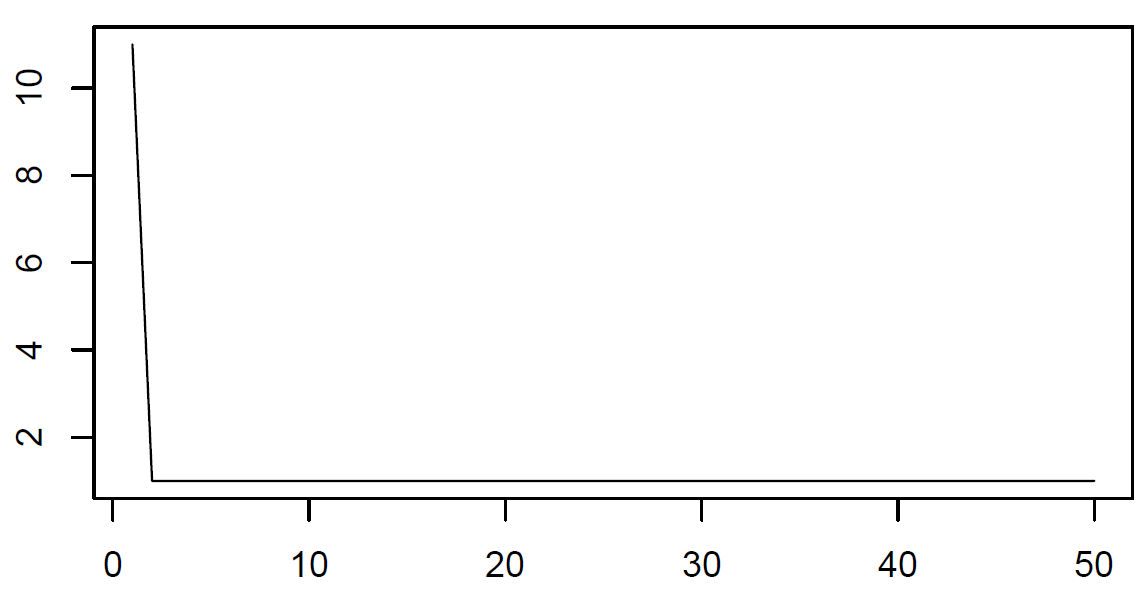
\includegraphics[, height = 2.2cm]{const_outl_graph_1.PNG}
%%         \caption{График $\Re(\tX{X})$.}
%%     \end{center}
%% \end{figure}
%\begin{figure}[H]
%     \begin{center}
%        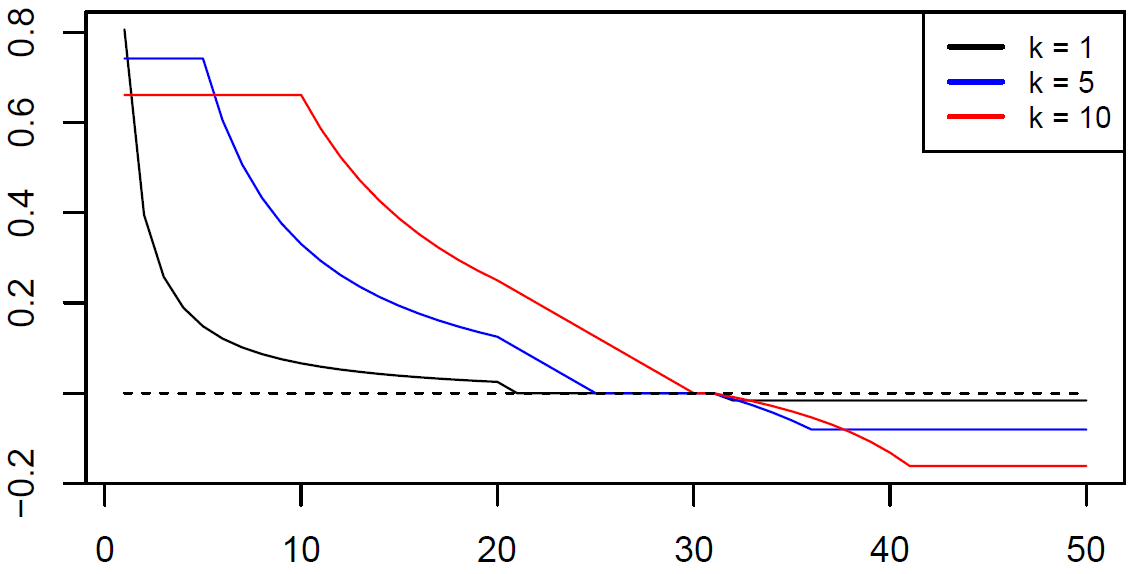
\includegraphics[, height = 5cm]{img/const_outl_err_1.PNG}
%        \caption{График $\Re(\text{CSSA-}\tX{F}^{(1)})$.}
%    \end{center}
%\end{figure}
%\end{frame}

%\begin{frame}{Выброс: График первого порядка для $L < k < K$}
%Рассмотрим
%$$s_l = 1 + \iu,$$
%$\tX{R}$~--- выброс $10 + \iu 10$ на позиции $k = 26$, $N = 51$, $L = 10, 20, 25$.
%
%% \begin{figure}[H]
%%     \begin{center}
%%         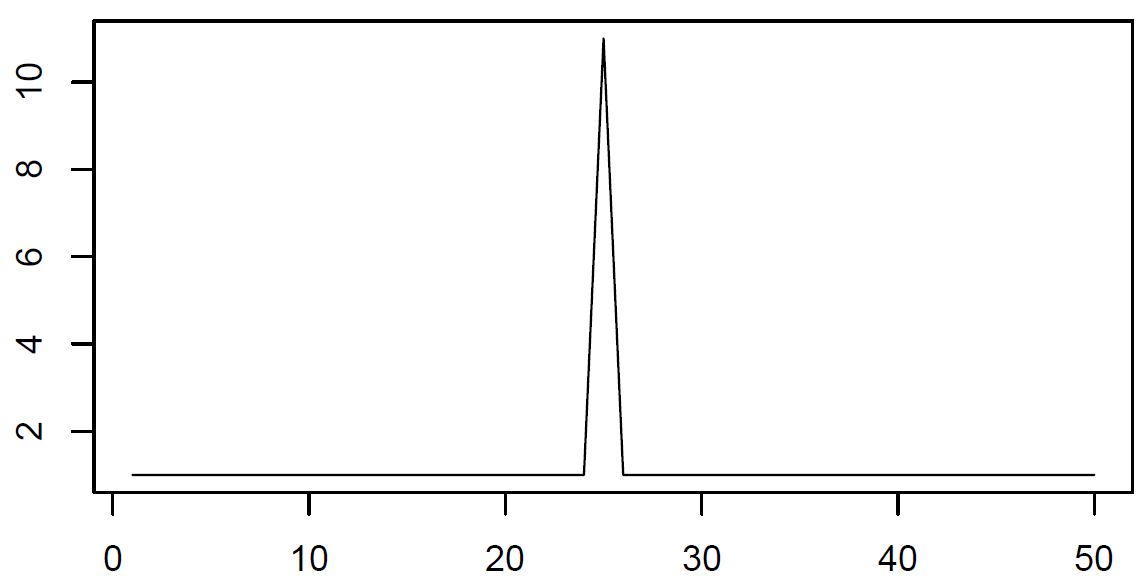
\includegraphics[, height = 2.2cm]{const_outl_graph_2.PNG}
%%         \caption{График $\Re(\tX{X})$.}
%%     \end{center}
%% \end{figure}
%\begin{figure}[H]
%     \begin{center}
%        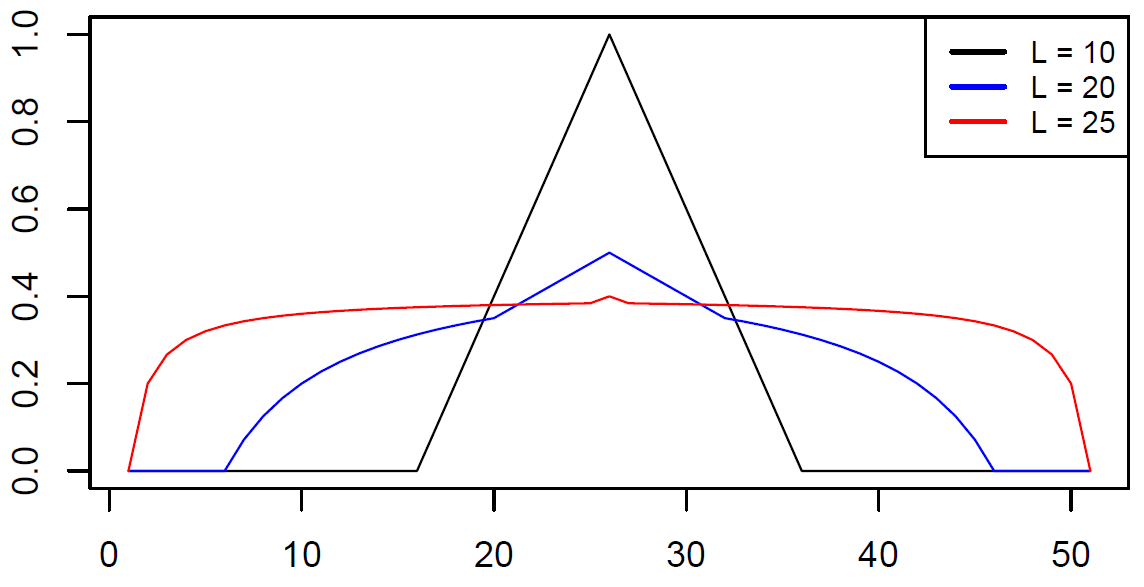
\includegraphics[, height = 5cm]{img/const_outl_err_2.PNG}
%        \caption{График $\Re(\text{CSSA-}\tX{F}^{(1)})$.}
%    \end{center}
%\end{figure}
%\end{frame}

\begin{frame}{Часть \RomanNumeralCaps{2}: Сравнение первого порядка и полной ошибок}
\alert{Зашумлённые синусоиды:} Численно было показано, первый порядок адекватно описывает полную ошибку.\\
\vspace{1em}
\alert{Константный сигнал с выбросом:} Численно было показано, первый порядок адекватно оценивает полную ошибку при $L = \alpha N$ для больших $N$. При малых $L$ это не так.\\
\vspace{1em}
\alert{Пример с выбросом:}
$$s_l = 1 + \iu,$$
$\tX{R}$~--- выброс $10 + \iu 10$ на позиции $k = L - 1$.

\begin{table}[H]
	\begin{center}
		\caption{Максимальное различие первого порядка и полной ошибок.}
		\label{tab:const_outl}
		\begin{tabular}{|c|c|c|c|c|}
			\hline
			$N$	& 50 & 100 & 400 & 1600 \\
			\hline
			$L = N / 2$ & 0.1313  & 0.0419  & 0.0033 & 0.0002 \\
			\hline
			$L = 20$ & 0.3074  & 0.1965  & 0.5655 & 0.6720 \\
			\hline
		\end{tabular}
	\end{center}
\end{table}

\end{frame}


\begin{frame}{Основные результаты}
    \begin{itemize}
    	\item \alert{Реадизации на R:} Робастные модификации были обобщены на комплексный случай. 
        \item \alert{Теория:} при совпадении траекторных пространств комплексного ряда первые порядки ошибок для CSSA и SSA совпадают.
        \item $s_l = A\cos(2 \pi\omega l + \phi_1) + \iu B\cos(2 \pi\omega l + \phi_2)$, сдвиг не $\pi / 2$
        $$\mathbb{D}(\text{CSSA-}f^{(1)}_l) = \mathbb{D}(\text{SSA-}f^{(1)}_{\Re, l}) + \mathbb{D}(\text{SSA-}f^{(1)}_{\Im, l}).$$
        $s_l = Ae^{\pm \iu(2 \pi\omega l + \phi_1)}$
        $$\mathbb{D}(\text{CSSA-}f^{(1)}_l) \stackrel{?}{=} \frac{1}{2}[\mathbb{D}(\text{SSA-}f^{(1)}_{\Re, l}) + \mathbb{D}(\text{SSA-}f^{(1)}_{\Im, l})].$$
        \item \alert{Теория:} для $s_l = c_1 + \iu c_2$ с выбросом была получена аналитическая формула первого порядка. При $L = \alpha N$ ошибка стремится к $0$.
        \item \alert{Численные эксперименты:} Рассмотрен вопрос приближения полной ошибки первым порядком.
    \end{itemize}
\end{frame}

%\begin{frame}{Список литературы}
%\begin{thebibliography}{10}
%{\small
%	\bibitem{Golyandina.etal2013}
%	N.~Golyandina, A.~Korobeynikov, A.~Shlemov, and K.~Usevich (2015)
%	\newblock Multivariate and {2D} extensions of singular spectrum analysis with
%	the {R}ssa package.
%	
%
%	\bibitem{Golyandina.etal2001}
%	N.~Golyandina, V.~Nekrutkin, and A.~Zhigljavsky (2001)
%	\newblock {\em Analysis of Time Series Structure: {SSA} and Related
%		Techniques}.
%
%	
%	\bibitem{Golyandina.Stepanov2005} 
%	Д.~Степанов, Н.~Голяндина (2005)
%	\newblock Варианты метода "Гусеница"{-SSA} для прогноза многомерных временных рядов.
%
%	\bibitem{Nekrutkin}
%	V.~Nekrutkin (2010)
%	\newblock Perturbation expansions of signal subspaces for long signals.
%
%	
%	\bibitem{NekrutkinPerp}
%	V.~Nekrutkin (2008)
%	\newblock Perturbations in SSA.
%
%	
%	\bibitem{Konstantinov}
%	А.~Константинов (2018)
%	\newblock Некоторые задачи анализа временных рядов.
%}	
%\end{thebibliography}
%\end{frame}

\end{document}
